\section{Simulation studies Paper V}
\begin{frame}
	\frametitle{Motivation}
	\begin{itemize}
		\item Test with a more detailed power plant model.
		\item Test with a more detailed power system model.
		\item Investigate some of the assumptions from previous papers.
	\end{itemize}
\end{frame}
\begin{frame}
	\frametitle{More detailed power system model}
	\begin{columns}
		\begin{column}{0.5\textwidth}
			\begin{itemize}
				\item Used the Nordic 44 test system in PSS/E.
			\end{itemize}
		\end{column}
		\begin{column}{0.5\textwidth}
			\begin{figure}
				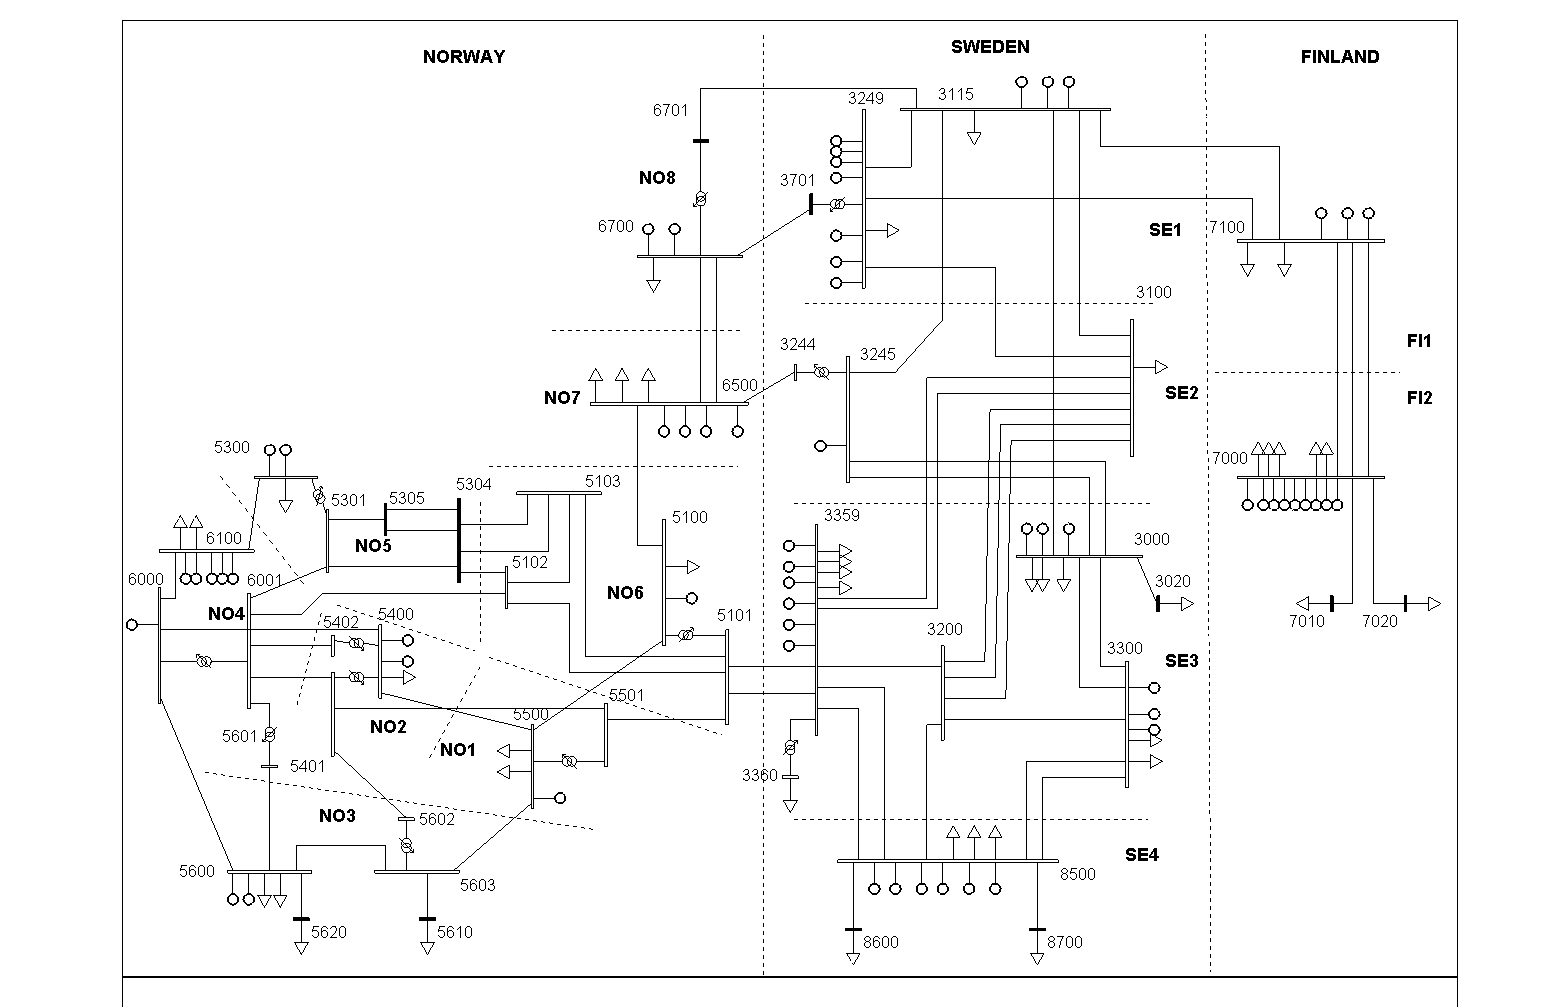
\includegraphics[width=\textwidth]{./pictures/Nordic44-Bilde}
			\end{figure}
		\end{column}
	\end{columns}
\end{frame}
\begin{frame}
	\frametitle{Test frequency assumption}
	\begin{columns}
		\begin{column}{0.3\textwidth}
			\begin{itemize}
				\item $f(s)$ is the derivative of the measured voltage.
				\item $\Delta \omega(s)$ is the rotational speed of the generator rotor.
				\item Increased the impedance between the generator and PMU.
				\item $100$ simulations for each impedance size-
			\end{itemize}
		\end{column}
		\begin{column}{0.7\textwidth}
			\includegraphics[width=0.9\textwidth]{./pictures/reactances.tikz}
			\includegraphics[width=0.8\textwidth]{./pictures/imp_change}
		\end{column}
	\end{columns}
\end{frame}
\begin{frame}
	\frametitle{Main contributions}
	\begin{itemize}
		\item Tested the methods with a more detailed power plant model.
		\item Tested the methods  with a more detailed power system model.
		\item Investigate some of the assumptions from previous papers.
	\end{itemize}
\end{frame}

